\documentclass[a4paper, 10pt]{article}

\usepackage{graphicx}
\usepackage{color}
\usepackage{tikz}
\usetikzlibrary{decorations.pathreplacing}
\usepackage{pgfplots}
\usepackage{pgf-umlsd}
\usepackage{ifthen}
\usepackage[]{fp}

\usetikzlibrary{matrix,patterns,spy,fit,calc}
\usepgfplotslibrary{groupplots}
\pgfplotsset{compat=newest}

\FPset{totalOffset}{0}

\begin{document}

\begin{figure}
	\centering
	\noindent\resizebox{\textwidth}{!}{
	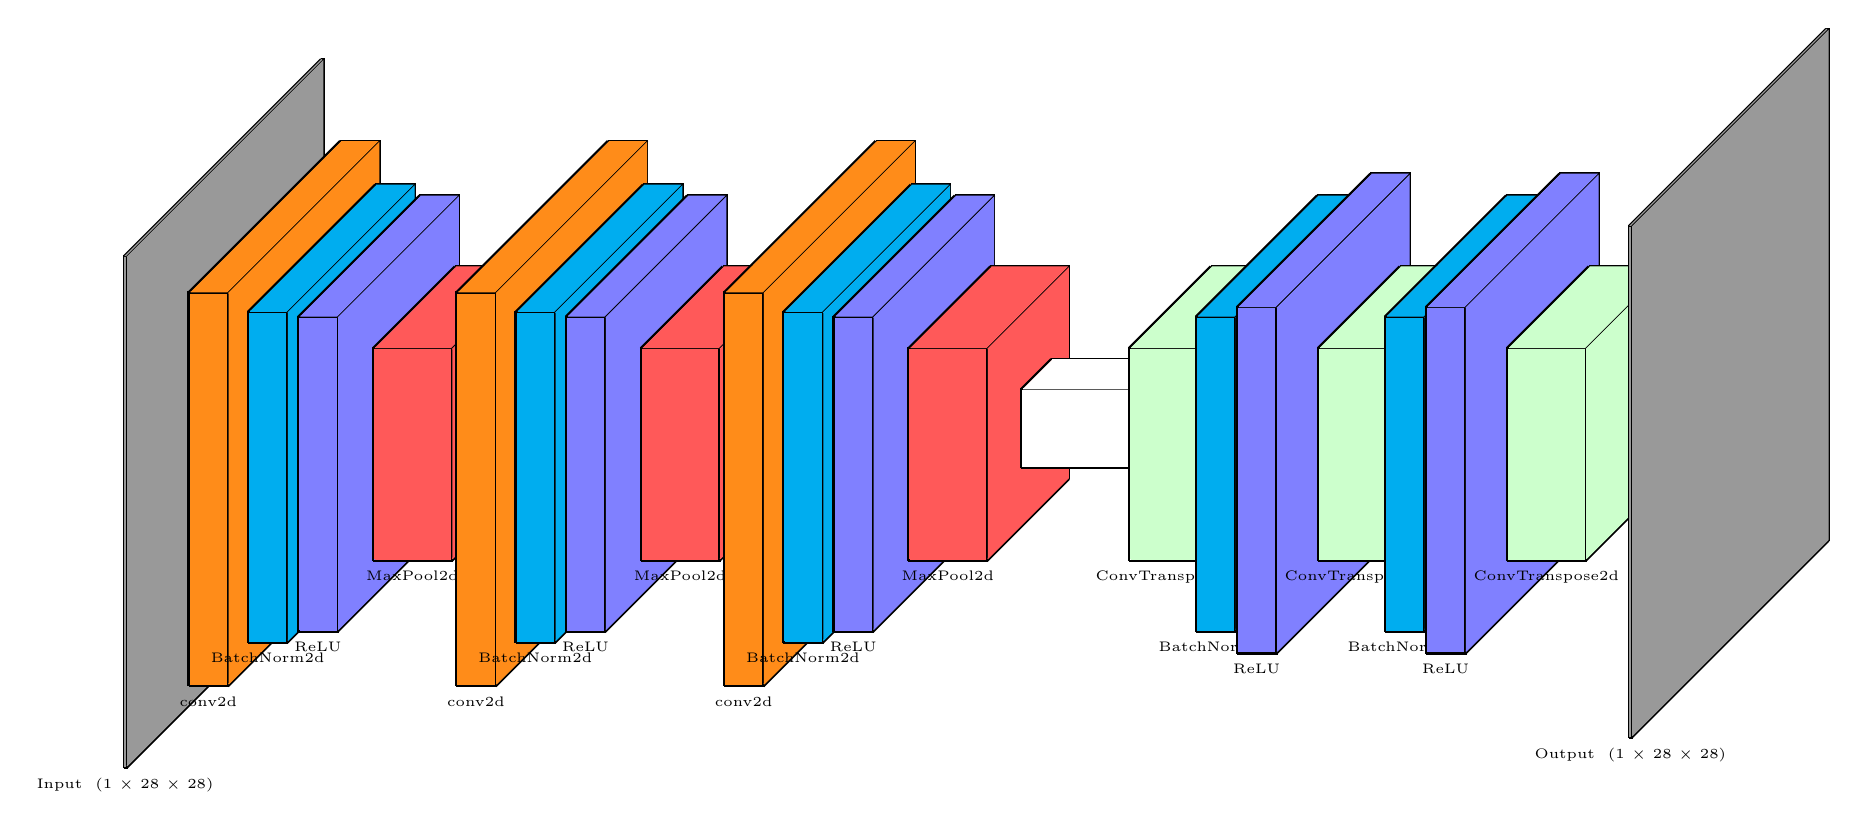
\begin{tikzpicture}
		%\draw[use as bounding box, transparent] (-1.8,-1.8) rectangle (17.2, 3.2);

		\newcommand{\networkLayer}[9]{
			
			\xdef\totalOffset{\totalOffset}
 			\ifthenelse{\equal{#8} {start}}
 			{\FPset{totalOffset}{0}}
 			{}
 			\FPeval\currentOffset{0+(totalOffset)+(#3)}

			\def\hw{#1} % Used to distinguish input resolution for current layer.
			\def\b{0.02}
			\def\c{#2} % Width of the cube to distinguish number of input channels for current layer.
			\def\x{\currentOffset} % X offset for current layer.
			\def\y{#4} % Y offset for current layer.
			\def\z{#5} % Z offset for current layer.
			\def\inText{#7}

            
            \coordinate (#8_front) at  (\x+\c  , \z      , \y);
            \coordinate (#8_back) at   (\x     , \z      , \y);
            \coordinate (#8_top) at    (\x+\c/2, \z+\hw/2, \y);
            \coordinate (#8_bottom) at (\x+\c/2, \z-\hw/2, \y);
            
 			
			\coordinate (blr) at (\c+\x,  -\hw/2+\z,  -\hw/2+\y); 
			\coordinate (bur) at (\c+\x,   \hw/2+\z,  -\hw/2+\y); 
			\coordinate (bul) at (0 +\x,   \hw/2+\z,  -\hw/2+\y);
			\coordinate (fll) at (0 +\x,  -\hw/2+\z,   \hw/2+\y); 
			\coordinate (flr) at (\c+\x,  -\hw/2+\z,   \hw/2+\y); 
			\coordinate (fur) at (\c+\x,   \hw/2+\z,   \hw/2+\y); 
			\coordinate (ful) at (0 +\x,   \hw/2+\z,   \hw/2+\y); 

            
            \ifthenelse{\equal{#9} {}}
 			{}{
 			    \foreach \val in #9
 			        \draw[line width=0.3mm] (\val)--(#8_back);
 			}
 			
			% Draw the layer body.
			% back plane
			\draw[line width=0.3mm](blr) -- (bur) -- (bul);
			% front plane
			\draw[line width=0.3mm](fll) -- (flr) node[midway,below] {\inText} -- (fur) -- (ful) -- (fll);
			\draw[line width=0.3mm](blr) -- (flr);
			\draw[line width=0.3mm](bur) -- (fur);
			\draw[line width=0.3mm](bul) -- (ful);

			% Recolor visible surfaces
			% front plane
			\filldraw[#6] ($(fll)+(\b,\b,0)$) -- ($(flr)+(-\b,\b,0)$) -- ($(fur)+(-\b,-\b,0)$) -- ($(ful)+(\b,-\b,0)$) -- ($(fll)+(\b,\b,0)$);
			\filldraw[#6] ($(ful)+(\b,0,-\b)$) -- ($(fur)+(-\b,0,-\b)$) -- ($(bur)+(-\b,0,\b)$) -- ($(bul)+(\b,0,\b)$);

			% Colored slice.
			\ifthenelse {\equal{#6} {}}{} 
			% Else, draw a colored slice.
			{\filldraw[#6] ($(flr)+(0,\b,-\b)$) -- ($(blr)+(0,\b,\b)$) -- ($(bur)+(0,-\b,\b)$) -- ($(fur)+(0,-\b,-\b)$);}

			\FPeval\totalOffset{0+(currentOffset)+\c}
		}
		
	%\networkLayer{2.0}{0.5}{0.0}{0.0}{2.5}{color=red!50}{}{start}{}
	%\networkLayer{2.0}{0.25}{1.5}{0.0}{0.0}{color=green!50}{}{bot}{{start_front}}
	%\networkLayer{2.0}{0.25}{0.15}{0.0}{0.0}{color=green!50}{}{}{}
	%\networkLayer{2.0}{0.5}{0.15}{0.0}{0.0}{color=green!50}{}{end}{}
	%\networkLayer{2.0}{0.5}{-(2.8)/2}{0.0}{5.0}{color=green!50}{}{top}{{start_front}}
	%\networkLayer{2.0}{0.5}{2.0}{0.0}{2.5}{color=blue!50}{}{add}{{end_front,top_front}}
	%\networkLayer{1.0}{0.5}{0.15}{0.0}{2.5}{color=blue!50}{}{}{}
	%\networkLayer{0.75}{0.5}{0.15}{0.0}{2.5}{color=blue!50}{}{}{}
	%\networkLayer{0.5}{0.5}{0.15}{0.0}{2.5}{color=blue!50}{}{}{}
			% INPUT
			
		\networkLayer{6.5}{0.03}{0.0}{0.0}{0.0}{color=gray!80}{\tiny{Input \ (1 $\times$ 28 $\times$ 28)}}{start}{}

		% ENCODER
		
		\networkLayer{5.0}{0.5}{0.5}{0.0}{0.0}{color=orange!90}{\tiny{conv2d}}{}{}    % S1
		\networkLayer{4.2}{0.5}{0.1}{0.0}{0.0}{color=cyan}{\tiny{BatchNorm2d} }{}{}        % S2
		\networkLayer{4.0}{0.5}{0.1}{0.0}{0.0}{color=blue!50}{\tiny{ReLU}}{}{}    % S1
		\networkLayer{2.7}{1.0}{0.2}{0.0}{0.0}{color=red!65}{\tiny{MaxPool2d}}{}{}        % S2
		%\networkLayer{2.0}{0.4}{0.1}{0.0}{0.0}{color=white}{conv}{}{}    % S1
		\networkLayer{5.0}{0.5}{0.5}{0.0}{0.0}{color=orange!90}{\tiny{conv2d}}{}{}    % S1
		\networkLayer{4.2}{0.5}{0.1}{0.0}{0.0}{color=cyan}{\tiny{BatchNorm2d} }{}{}        % S2
		\networkLayer{4.0}{0.5}{0.1}{0.0}{0.0}{color=blue!50}{\tiny{ReLU}}{}{}    % S1
		\networkLayer{2.7}{1.0}{0.2}{0.0}{0.0}{color=red!65}{\tiny{MaxPool2d}}{}{}        % S2
		%\networkLayer{2.0}{0.4}{0.1}{0.0}{0.0}{color=white}{conv}{}{}    % S1
		\networkLayer{5.0}{0.5}{0.5}{0.0}{0.0}{color=orange!90}{\tiny{conv2d}}{}{}    % S1
		\networkLayer{4.2}{0.5}{0.1}{0.0}{0.0}{color=cyan}{\tiny{BatchNorm2d} }{}{}        % S2
		\networkLayer{4.0}{0.5}{0.1}{0.0}{0.0}{color=blue!50}{\tiny{ReLU}}{}{}    % S1
		\networkLayer{2.7}{1.0}{0.2}{0.0}{0.0}{color=red!65}{\tiny{MaxPool2d}}{}{}        % S2
		
		%\networkLayer{2.0}{0.4}{0.1}{0.0}{0.0}{color=white}{}{}{}        % S2
		%\networkLayer{1.5}{0.8}{0.1}{0.0}{0.0}{color=white}{conv}{}{}    % S1
		%\networkLayer{1.5}{0.8}{0.1}{0.0}{0.0}{color=white}{}{}{}        % S2
		%\networkLayer{1.0}{1.5}{0.1}{0.0}{0.0}{color=white}{conv}{}{}    % S1
		\networkLayer{1.0}{1.5}{0.1}{0.0}{0.0}{color=white}{}{mid}{}        % S2

		%\networkLayer{1.0}{0.5}{1.5}{0.0}{-1.5}{color=green!50}{}{bot}{{mid_front}}
		%\networkLayer{1.0}{0.5}{-0.5}{0.0}{1.5}{color=green!50}{}{top}{{mid_front}}
		%\networkLayer{1.0}{0.5}{1.5}{0.0}{0.0}{color=blue!50}{sum}{}{{bot_front,top_front}}

		% DECODER
		%\networkLayer{1.0}{1.5}{0.1}{0.0}{0.0}{color=white}{deconv}{}{} % S1
		%\networkLayer{1.0}{1.5}{0.1}{0.0}{0.0}{color=white}{}{}{}       % S2
		%\networkLayer{1.5}{0.8}{0.1}{0.0}{0.0}{color=white}{deconv}{}{} % S1
		\networkLayer{2.7}{1.0}{0.2}{0.0}{0.0}{color=green!20}{\tiny{ConvTranspose2d}}{}{} 
		\networkLayer{4.0}{0.5}{0.1}{0.0}{0.0}{color=cyan}{\tiny{BatchNorm2d} }{}{}        % S2
		\networkLayer{4.4}{0.5}{0.1}{0.0}{0.0}{color=blue!50}{\tiny{ReLU}}{}{}    % S1
		%\networkLayer{2.0}{0.4}{0.1}{0.0}{0.0}{color=white}{}{}{}       % S1
		\networkLayer{2.7}{1.0}{0.2}{0.0}{0.0}{color=green!20}{\tiny{ConvTranspose2d}}{}{} 
		\networkLayer{4.0}{0.5}{0.1}{0.0}{0.0}{color=cyan}{\tiny{BatchNorm2d} }{}{}        % S2
		\networkLayer{4.4}{0.5}{0.1}{0.0}{0.0}{color=blue!50}{\tiny{ReLU}}{}{}    % S1
		\networkLayer{2.7}{1.0}{0.2}{0.0}{0.0}{color=green!20}{\tiny{ConvTranspose2d}}{}{} 
		%\networkLayer{2.0}{0.4}{0.1}{0.0}{0.0}{color=white}{}{}{}       % S2
		%\networkLayer{2.5}{0.2}{0.1}{0.0}{0.0}{color=white}{}{}{}       % S1
		%\networkLayer{2.5}{0.2}{0.1}{0.0}{0.0}{color=white}{}{}{}       % S2
		%\networkLayer{3.0}{0.1}{0.1}{0.0}{0.0}{color=white}{}{}{}       % S1
		%\networkLayer{3.0}{0.1}{0.1}{0.0}{0.0}{color=white}{}{}{}       % S2

		% OUTPUT
		\networkLayer{6.5}{0.03}{0.9}{-1.0}{0.0}{color=gray!80}{\tiny{Output \ (1 $\times$ 28 $\times$ 28)}}{}{}          
	\end{tikzpicture}
	}
	\caption{Ejemplo de  CNN.}
	\label{fig:cnn}
\end{figure}

\end{document}